\section{Theoretical Algebra}
In this section, a collection of XQuery query examples and their translation to
relational algebra is presented. The translation is done manually using the
``Tainting Dependencies'' method described in section
\ref{sect:trans:taintingDependencies}. For the sake of brevity, only the
rules used throughout the translation will be noted. Intermediate results will
not be included.

Generell struktur:
- Sp\oe rring
- Semantikk (resultat)
- Translasjon
- Mellomregninger? (naaii..)

\subsection{Extensive FLWOR}
This example will illustrate the translation of a more complex FLWOR expression.

\subsubsection{Query premise}
\begin{figure}[htp]
\begin{center}
\begin{Verbatim}
for $a in (1,2,3) let $b := 2
  where $a gt $b
  order by $a
  return ($a, $b)
\end{Verbatim}
  \caption{Extensive FLWOR expression, showcasing for-, let-, where-, orderby-,
  and return-clauses}
  \label{fig:results:query_ext_flwor}
\end{center}
\end{figure}

\subsubsection{Translation process}
The translation process in its entirety is shown step by step in appendix
\ref{appendix:transl:ext_flwor}, page \pageref{appendix:transl:ext_flwor}.

\subsubsection{Result}
The result of the translation is shown in figure
\ref{fig:results:query_ext_flwor_result}.

\begin{figure}[htp]
\begin{center}
  \begin{Verbatim}
project(value=l.value, anumb;
  numberate(index, [r.value, index], [anumb];
    hhjoin([l.anumb], [r.anumb], [l.value, r.value, anumb];
      hhjoin([],[], [l.value, anumb];
        numberate(index,[sprIdx,index],[];
          union(;
            project([anumb = index, index = 1, value];
              make(name:=[index, value], [1,2,3], [1,2,3])),
            make(name:=[value],2))),
        select(xqBoolean(value);
          project(index=1, value=gt(r.value, l.value), anumb;
            hhjoin([l.anumb], [r.anumb], [l.value, r.value, anumb];
              project([anumb = index, index = 1, value];
                make(name:=[index, value], [1,2,3], [1,2,3])),
              make(name:=[value],2)))),
      project([anumb = index, index = 1, value];
        make(name:=[index, value], [1,2,3], [1,2,3])))))
  \end{Verbatim}
  \caption{Complete translation of expression in figure
  \ref{fig:results:query_ext_flwor}}
  \label{fig:results:query_ext_flwor_result}
\end{center}
\end{figure}

The operator tree in figure \ref{fig:results:query_ext_flwor_result} can be
converted to the DAG seen in figure \ref{fig:results:query_ext_flwor_dag}.

\newpage

\begin{figure}[!htp]
%\begin{center}
  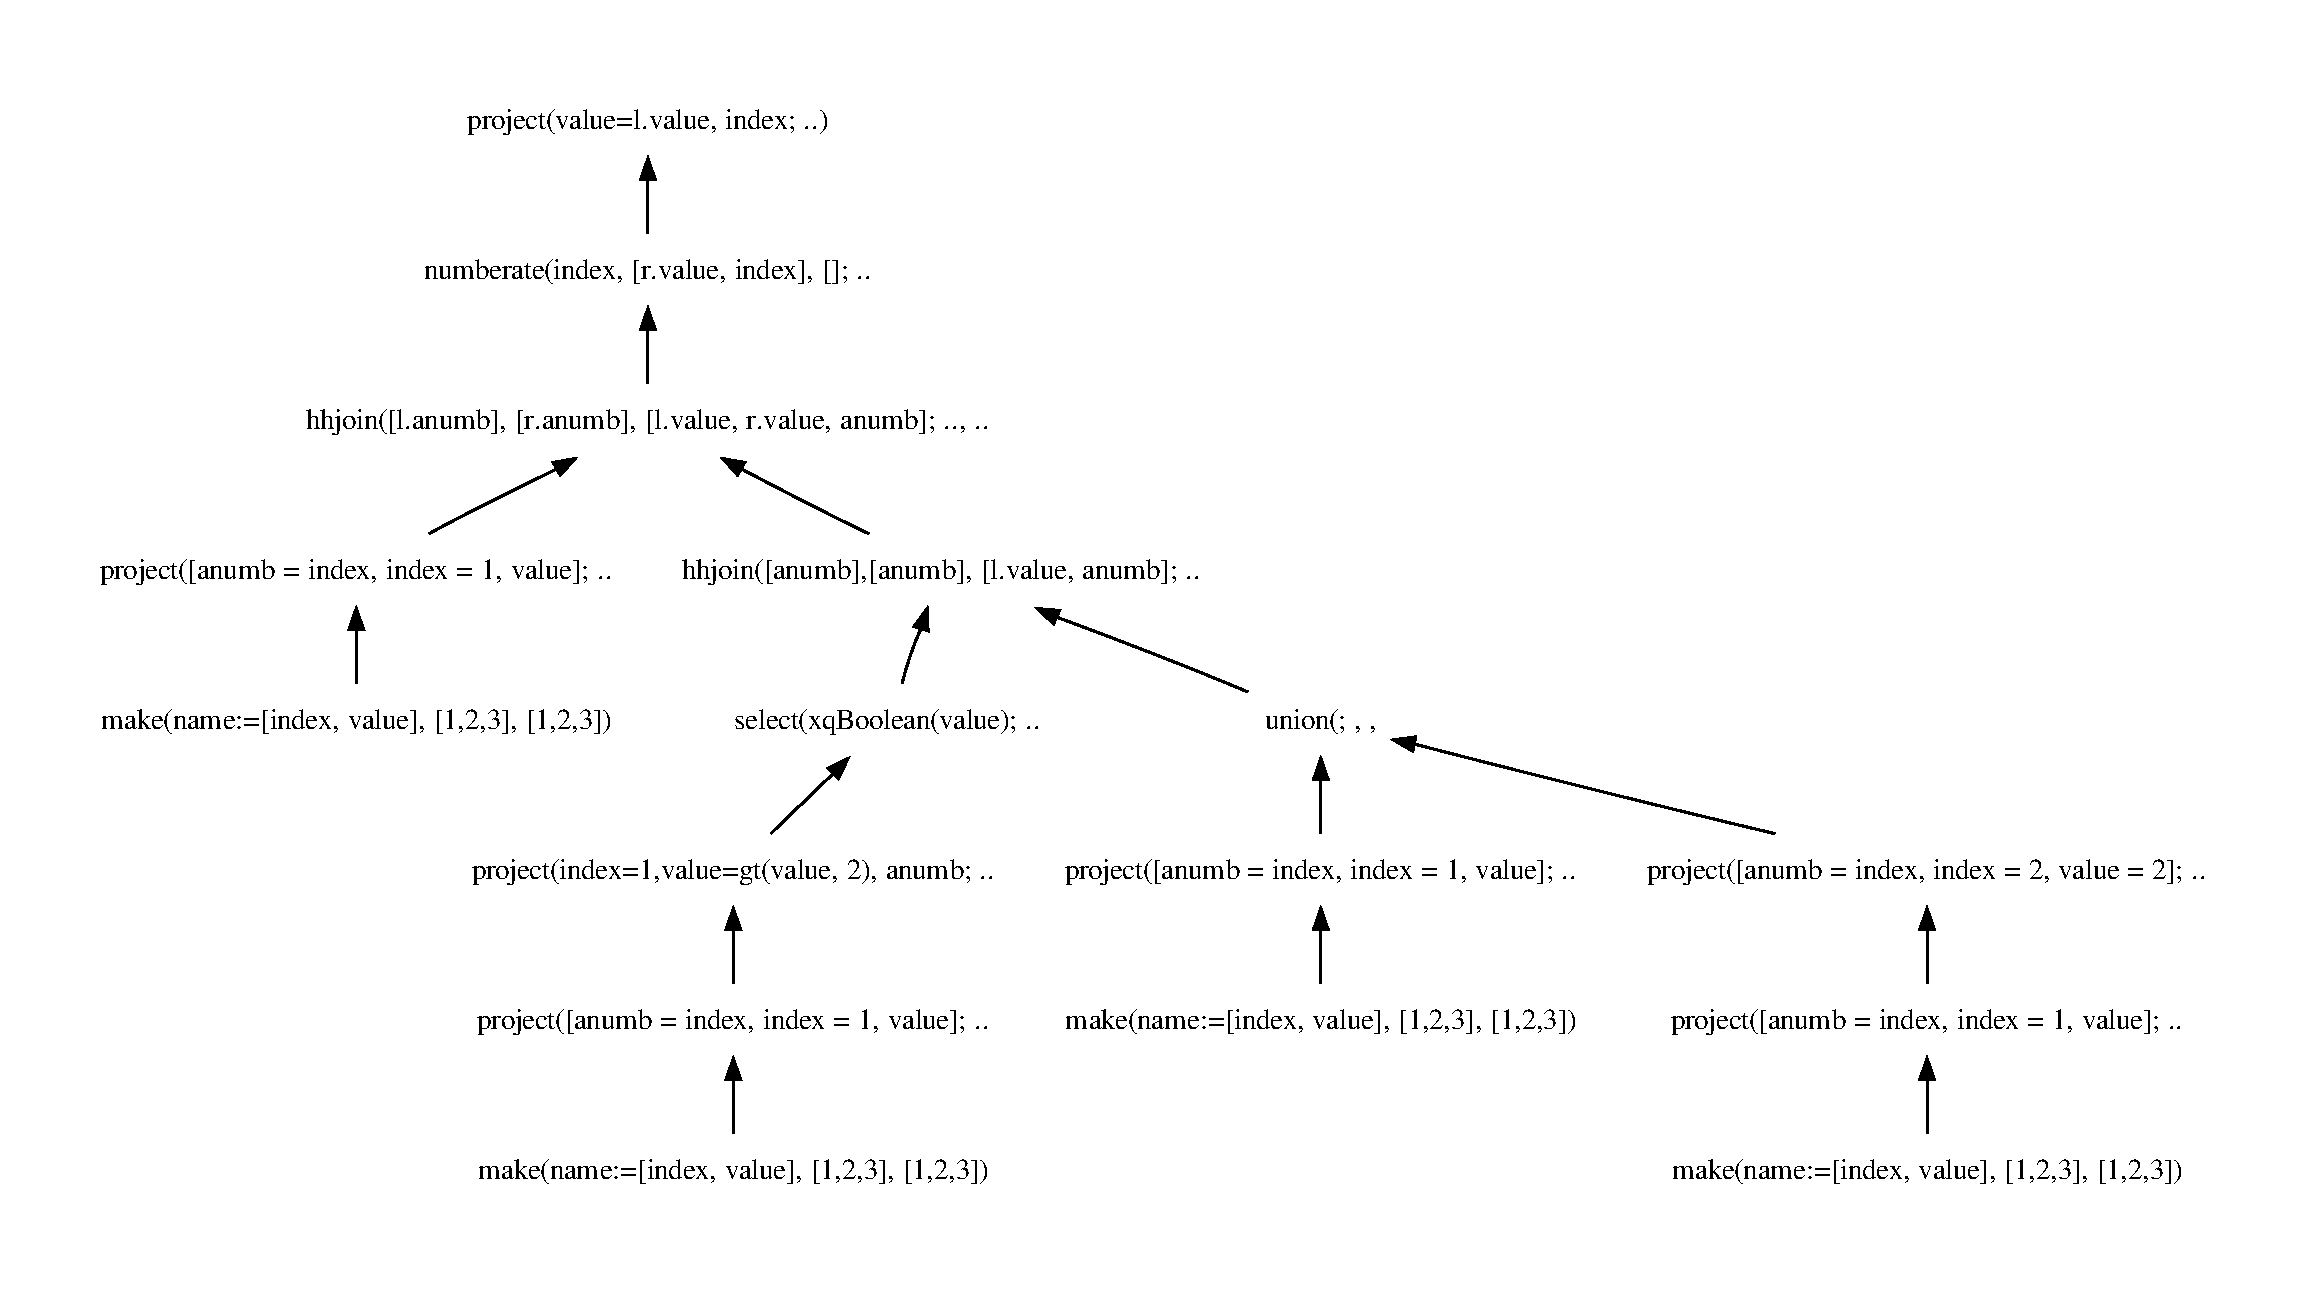
\includegraphics[scale=0.7]{img/graphs/ext_flwor}
  \caption{DAG representation of operator tree in figure
  \ref{fig:results:query_ext_flwor_result}}
  \label{fig:results:query_ext_flwor_dag}
%\end{center}
\end{figure}

\subsection{Path expression with predicate}
\begin{Verbatim}
/a/b[@id = 2] ?
\end{Verbatim}

\subsection{If-then-else}
\subsubsection{Query premise}
\begin{figure}[!htp]
\begin{center}
\begin{Verbatim}
for $a in (1,2,3) return 
  if $a > 2 then $a else 3
\end{Verbatim}
  \caption{If-then-else query premise}
  \label{fig:results:query_ifthenelse}
\end{center}
\end{figure}

\subsubsection{Translation process}
The translation process in its entirety is shown step by step in appendix
\ref{appendix:transl:ifthenelse}, page \pageref{appendix:transl:ifthenelse}.

\subsubsection{Result}
Omg


\section{Algebra Generated By Implementation}
In this section, a collection of trivial queries are translated to relational
algebra using the implemented proof of concept described in chapter
\ref{chapter:implementation}. Naturally, this implementation also uses the
``Tainting Dependencies'' method, however the results from these translations
can also be used in a comparison with loop lifting.

\subsection{FLWOR}


\subsection{Sequence construction}

\begin{itemize}
  \item to-tre større eksempler som benytter seg av Tainted Dependencies [skal
  disse v\ae re med mellomregninger og slikt? huff]
  \item et eksempel generert av implementasjonen [bare ett?]
\end{itemize}